\documentclass[9pt]{beamer}
\usetheme{Madrid}
\usefonttheme{serif}

\usepackage{fontspec}
% надёжный шрифт с кириллицей (работает в Overleaf)
\setmainfont{Libertinus Serif}[Ligatures=TeX]
\setsansfont{Libertinus Sans}[Ligatures=TeX]
\newfontfamily\cyrillicfont{Libertinus Serif}
\newfontfamily\cyrillicfontsf{Libertinus Sans}
\usepackage{polyglossia}
\setmainlanguage{russian}
\setotherlanguage{english}

\usepackage{amsmath}
\usepackage{amsfonts}
\usepackage{amssymb}
\usepackage{graphicx}
\usepackage{microtype}

\DeclareMathOperator{\sen}{sen}
% \DeclareMathOperator{\tg}{tg}

\setbeamertemplate{caption}[numbered]

% --- Информация о презентации ---
\author[Автор]{Чиняев Владимир Николаевич}
\title{Введение}
\newcommand{\coursename}{Введение в маневрирование} % <-- Поставь здесь нужное название курса
\setbeamertemplate{navigation symbols}{} 
\institute[]{Московский физико технический институт} 
\date{9 сентября 2025 г.} 

\bibliographystyle{apalike}

% --- Кастомная нижняя синяя полоска: курс слева, номер слайда справа ---
\setbeamertemplate{footline}{
  \leavevmode%
  \begin{beamercolorbox}[wd=\paperwidth,ht=2ex,dp=1ex]{palette primary}
    \hspace{0.4cm}\usebeamerfont{footline}\coursename\hfill\usebeamerfont{footline}\insertframenumber\hspace{0.4cm}
  \end{beamercolorbox}%
}

% Чтобы убрать лишние отступы в footer-шрифте (опционально)
\setbeamerfont{footline}{size=\small}

\begin{document}

\begin{frame}
\titlepage
\end{frame}

\begin{frame}
\centering

\includegraphics[height=0.70\textheight,keepaspectratio]{images/1/qr.png}
\end{frame}

\begin{frame}{Что такое маневрирование?}
Маневрирование - целенаправленное изменение параметров орбиты космического аппарата (КА) с помощью двигательной установки (ДУ).

Задачи, решаемые с помощью маневрирования:
\begin{itemize}
    \item Переход;
    \item Встреча;
    \item Уклонение;
    \item Формирование конфигурации спутниковых систем; 
    \item Поддержание конфигурации спутниковых систем;
    \item и тд.
\end{itemize}
\end{frame}

\begin{frame}{Кеплеровы элементы орбиты}
\begin{columns}[T,onlytextwidth]
  % левая колонка: картинка
  \begin{column}{0.48\textwidth}
    \centering
    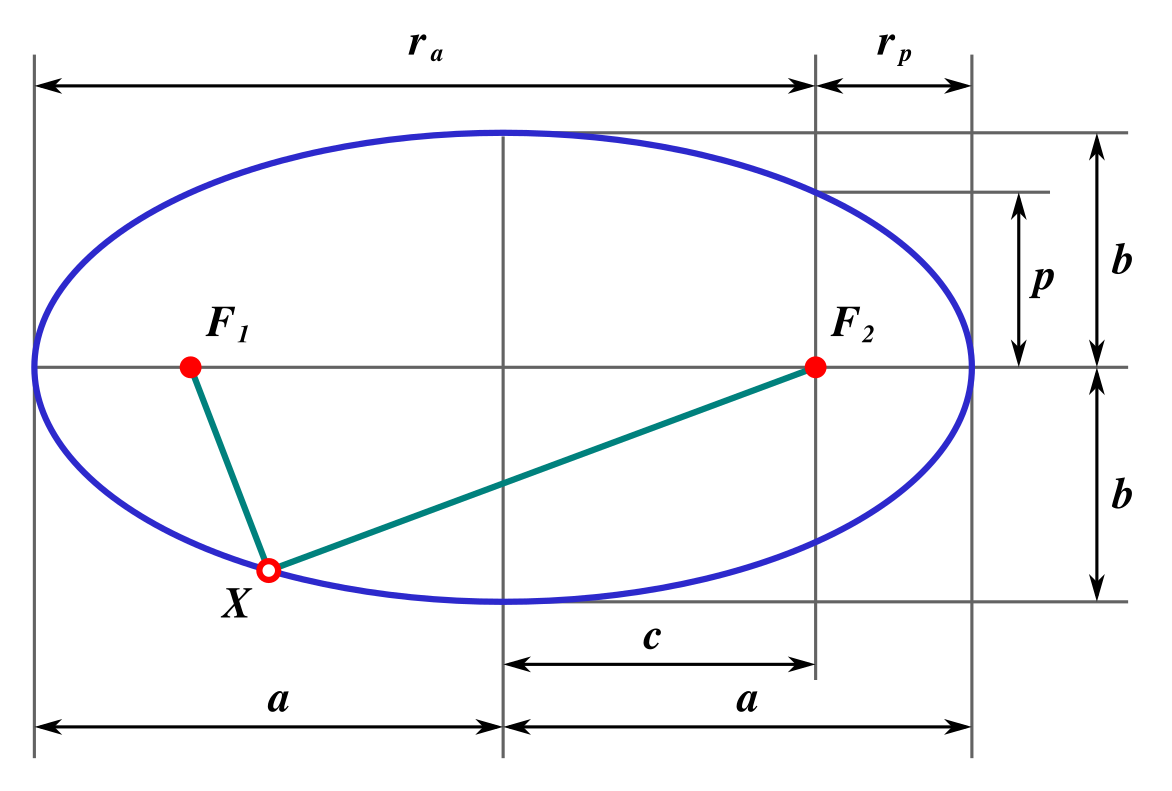
\includegraphics[height=0.40\textheight,keepaspectratio]{images/1/ellipse.png}
    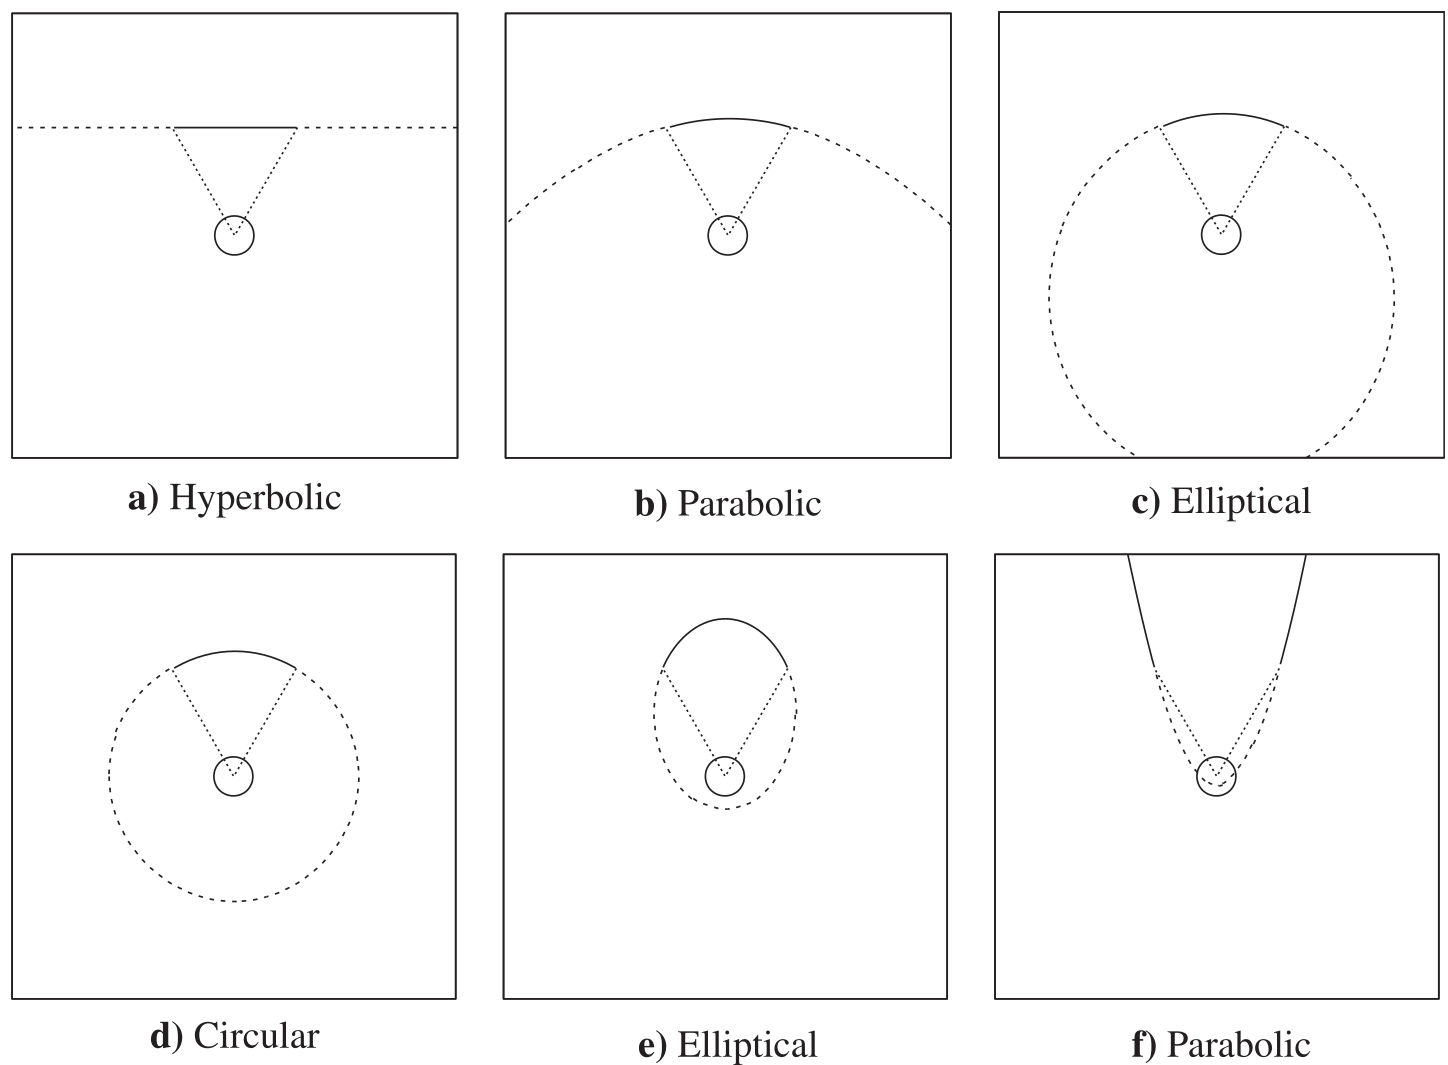
\includegraphics[height=0.40\textheight,keepaspectratio]{images/1/types.png}
  \end{column}

  % правая колонка: список
  \begin{column}{0.52\textwidth}
    \begin{itemize}
        \item Большая полуось $a$, [м] \\
            $a \in (0; +\infty)$
        \item Эксцентриситет $e$, [1] \\
            $e = 0$ --- круговая орбита; \\
            $e \in (0; 1)$ --- эллиптическая орбита; \\
            $e = 1$ --- параболическая орбита; \\
            $e \in (1; +\infty)$ --- гиперболическая орбита; \\
            $e = +\infty$ --- прямая.
        \item Аргумент перицентра $\omega$, [рад] \\
            $\omega \in [0; 2 \pi)$
    \end{itemize}
  \end{column}
\end{columns}
\end{frame}

\begin{frame}{Кеплеровы элементы орбиты}
\begin{columns}[T,onlytextwidth]
  % левая колонка: картинка
  \begin{column}{0.48\textwidth}
    \centering
    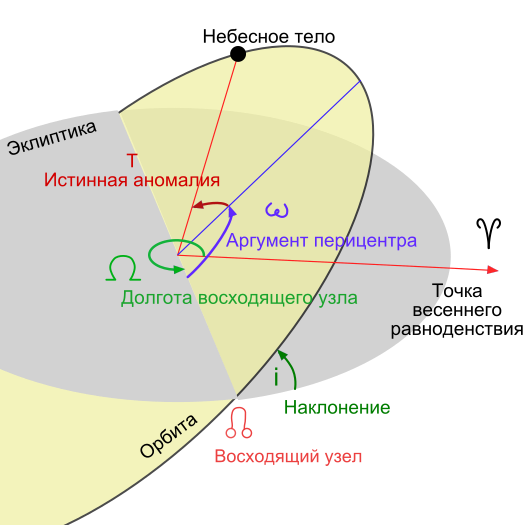
\includegraphics[height=0.70\textheight,keepaspectratio]{images/1/kepler.png}
    \label{fig:kep_els}
  \end{column}

  % правая колонка: список
  \begin{column}{0.52\textwidth}
    \begin{itemize}
        \item Наклонение $i$, [рад] \\
            $i \in [0; 2 \pi)$
        \item Долгота восходящего узла $\Omega$, [рад] \\
            $\Omega \in [0; 2 \pi)$
        \item Истинная аномалия $\nu$, [рад] \\
            $\nu \in [0; 2 \pi)$
    \end{itemize}
  \end{column}
\end{columns}
\end{frame}

\begin{frame}{Кеплеровы элементы орбиты}
\begin{columns}[T,onlytextwidth]
  % левая колонка: картинка
  \begin{column}{0.48\textwidth}
    \centering
    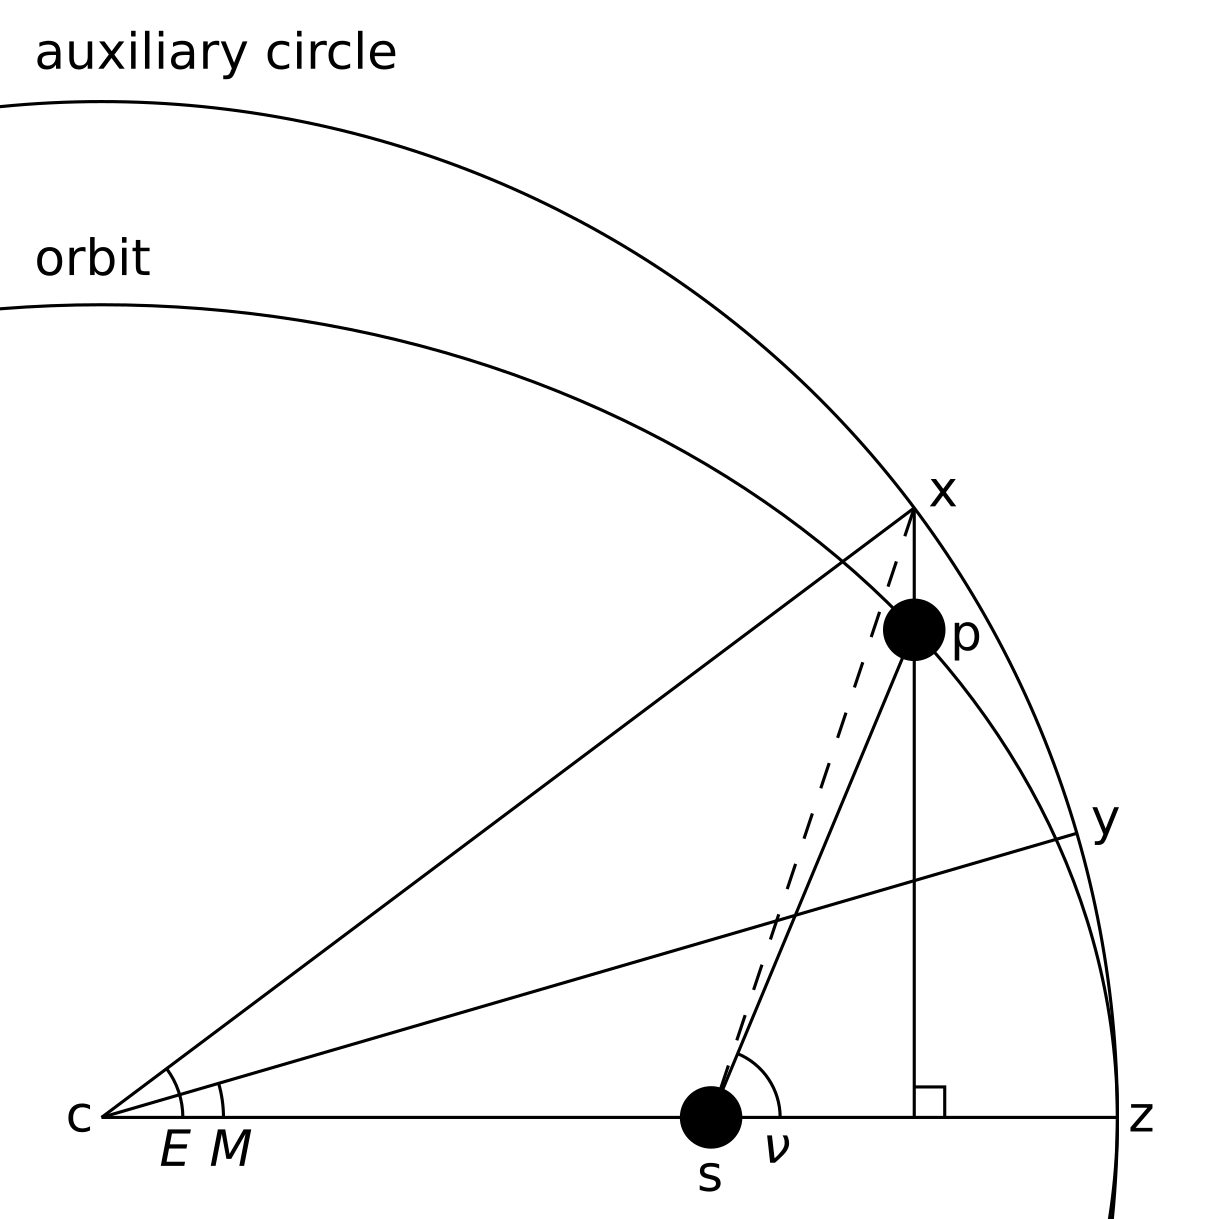
\includegraphics[height=0.70\textheight,keepaspectratio]{images/1/anomalies.png}
    \label{fig:kep_els}
  \end{column}

  % правая колонка: список
  \begin{column}{0.52\textwidth}
    Существуют другие варианты быстро меняющихся элементов:
    \begin{itemize}
        \item Эксцентрическая аномалия $E$, [рад]; \\
            \begin{equation*}
                \sin E = \frac{\sin \nu \sqrt{1 - e^2}}{1 + e \cos \nu},
            \end{equation*}
            \begin{equation*}
                \cos E = \frac{e + \cos \nu}{1 + e \cos \nu}.
            \end{equation*}
        \item Средняя аномалия $M$, [рад]; \\
            \begin{equation*}
                M = E - e \sin E,
            \end{equation*}
            \begin{equation*}
                E_{k + 1} = E_k + \frac{M - E_k + e \sin E_k}{1 - e \cos E_k}.
            \end{equation*}
        \item Истинный аргумент широты $u = \nu + \Omega$, [рад];
        \item Средний аргумент широты $\overline{u} = M + \Omega$, [рад].
    \end{itemize}
  \end{column}
\end{columns}
\end{frame}

\begin{frame}{Кеплеровы элементы орбиты}
\begin{columns}[T,onlytextwidth]
  % левая колонка: картинка
  \begin{column}{0.50\textwidth}
    Плюсы:
    \begin{itemize}
        \item \textbf{Физическая и геометрическая интерпретируемость.} \\
        Это облегчает диагностику и принятие решений при проектировании и анализе. Позволяют отдельно судить об о форме орбиты ($ a, e$), её ориентации ($ \omega, \Omega, i$) и положении на орбите ($\nu, M, E$).

        \item \textbf{Удобны для миссионного/набросочного планирования.} \\
        Позволяют быстро оценить различные характеристики орбиты.

        \item \textbf{Стандарты и совместимость} \\
        Многие справочники, каталоги (TLE) и инструменты используют элементы, поэтому удобно для обмена данными.
        
    \end{itemize}
  \end{column}

  % правая колонка: список
  \begin{column}{0.50\textwidth}
    Минусы:
    \begin{itemize}
        \item \textbf{Имеют вырождения.} \\ 
        При $e \rightarrow 0$ аргумент перицентра $\omega$ не определён. \\
        При $i \rightarrow 0$ долгота восходящего узла $\Omega$ не определёна.
        Эти вырождения приводят к проблемам в численных алгоритмах.
    \end{itemize}
  \end{column}
\end{columns}
\end{frame}

\begin{frame}{Модифицированные равноденственные элементы}
\begin{equation*}
    \begin{aligned}
        a &= a \\
        h &= e \sin (\omega + I \Omega)\\
        k &= e \cos (\omega + I \Omega)\\
        p &= \left( \tan \frac{i}{2} \right)^I \sin \Omega\\
        q &= \left( \tan \frac{i}{2} \right)^I \cos \Omega\\
        \lambda &= M + \omega + I \Omega
    \end{aligned}
\end{equation*}
где $I$ --- ретроградный фактор, значение которого выбирается в зависимости от наклонения: для проградных орбит (\(i \le \pi/2\)) $I = 1$, для ретроградных орбит (\(i > \pi/2\)) $I = -1$. \\
Для проградного набора элементов:
\begin{equation*}
    \lim_{i \rightarrow \pi} \sqrt{p^2 + q^2} = \infty.
\end{equation*}
Для ретроградного набора элементов:
\begin{equation*}
    \lim_{i \rightarrow 0} \sqrt{p^2 + q^2} = \infty.
\end{equation*}
\end{frame}

\begin{frame}{Орбитальная система координат}
\begin{columns}[T,onlytextwidth]
  % левая колонка: картинка
  \begin{column}{0.48\textwidth}
    \centering
    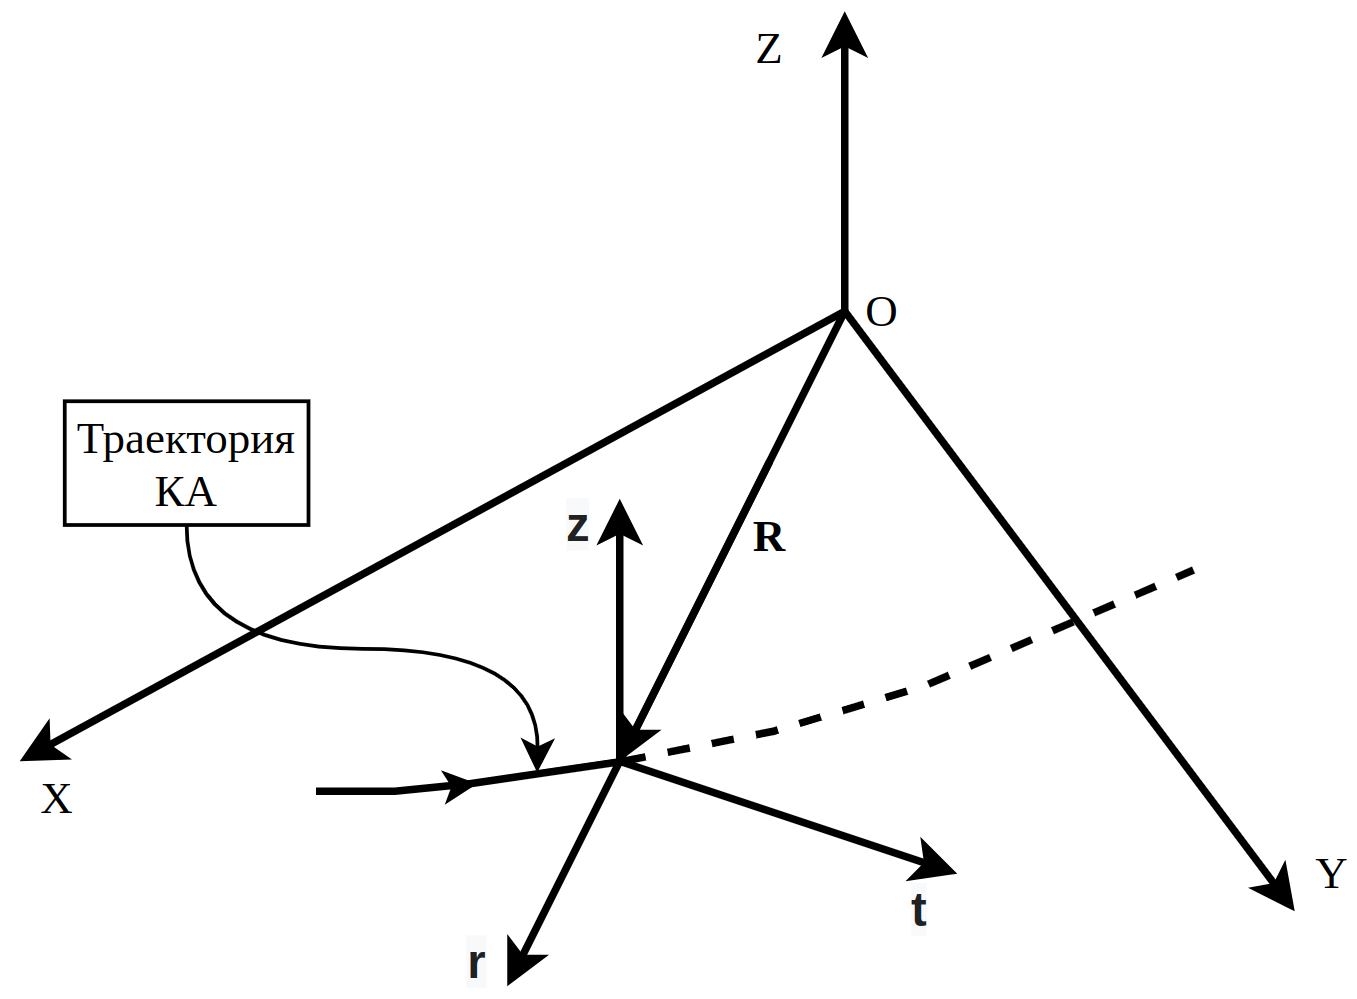
\includegraphics[height=0.50\textheight,keepaspectratio]{images/1/orbital_sk.png}
    \label{fig:orb_sk}
  \end{column}

  % правая колонка: список
  \begin{column}{0.52\textwidth}
    Определим её следующим образом:
    \begin{itemize}
        \item Начало отсчёта $O$ --- центр масс КА;
        \item Радиальный вектор $\mathbf{r}$ --- сонаправлен радиус-вектору КА;
        \item Трансверсальный вектор $\mathbf{t}$ --- перпендикулярен радиус-вектору КА, находится в плоскости орбиты и направлен в сторону движения;
        \item Нормальный вектор $\mathbf{z}$ --- дополняет систему векторов до правой тройки.
    \end{itemize}
  \end{column}
\end{columns}
\end{frame}

\begin{frame}{Уравнение движения КА}
Уравнение движения КА
\begin{equation*}
    \dot{\mathbf{y}} = \mathbf{f}(t, \mathbf{y}) + \mathbf{u}(t),
\end{equation*}
где $\mathbf{y}(t) = \left( a(t), e(t), i(t), \omega(t), \Omega(t), \nu(t) \right)^T$ --- вектор состояния, $\mathbf{f}(t, \mathbf{y})$ --- правая часть пассивного движения, $\mathbf{u}(t)$ --- управляющая функция.

Функция $\mathbf{f}(t, \mathbf{y})$ может быть представлена в следующем виде:
\begin{equation*}
    \mathbf{f}(t, \mathbf{y}) = B(\mathbf{y}) \mathbf{\Delta},
\end{equation*}
где $B(\mathbf{y})$ --- матрица производных правой части по возмущающим ускорениям, а $\mathbf{\Delta} = (\Delta_r, \Delta_t, \Delta_z)^T$ --- проекции возмущающих ускорений на оси орбитальной СК.
\end{frame}

\begin{frame}{Силы, действующие на КА}
В действительности на КА действует целый спектр сил:
\begin{equation*}
    \mathbf{F}_{\Sigma} = \mathbf{F}_{central} + \mathbf{F}_{perturb}, 
\end{equation*}
где 
\begin{equation*}
    \mathbf{F}_{perturb} = \mathbf{F}_{grav} + \mathbf{F}_{drag} + \mathbf{F}_{others} + \mathbf{F}_{rad}.
\end{equation*}
Тогда можно записать 
\begin{equation*}
    \mathbf{F}_{\Sigma} = m \mathbf{\Delta}.
\end{equation*}
\end{frame}

\begin{frame}{Реальное движение КА}
\begin{figure}[h!]
    \centering
    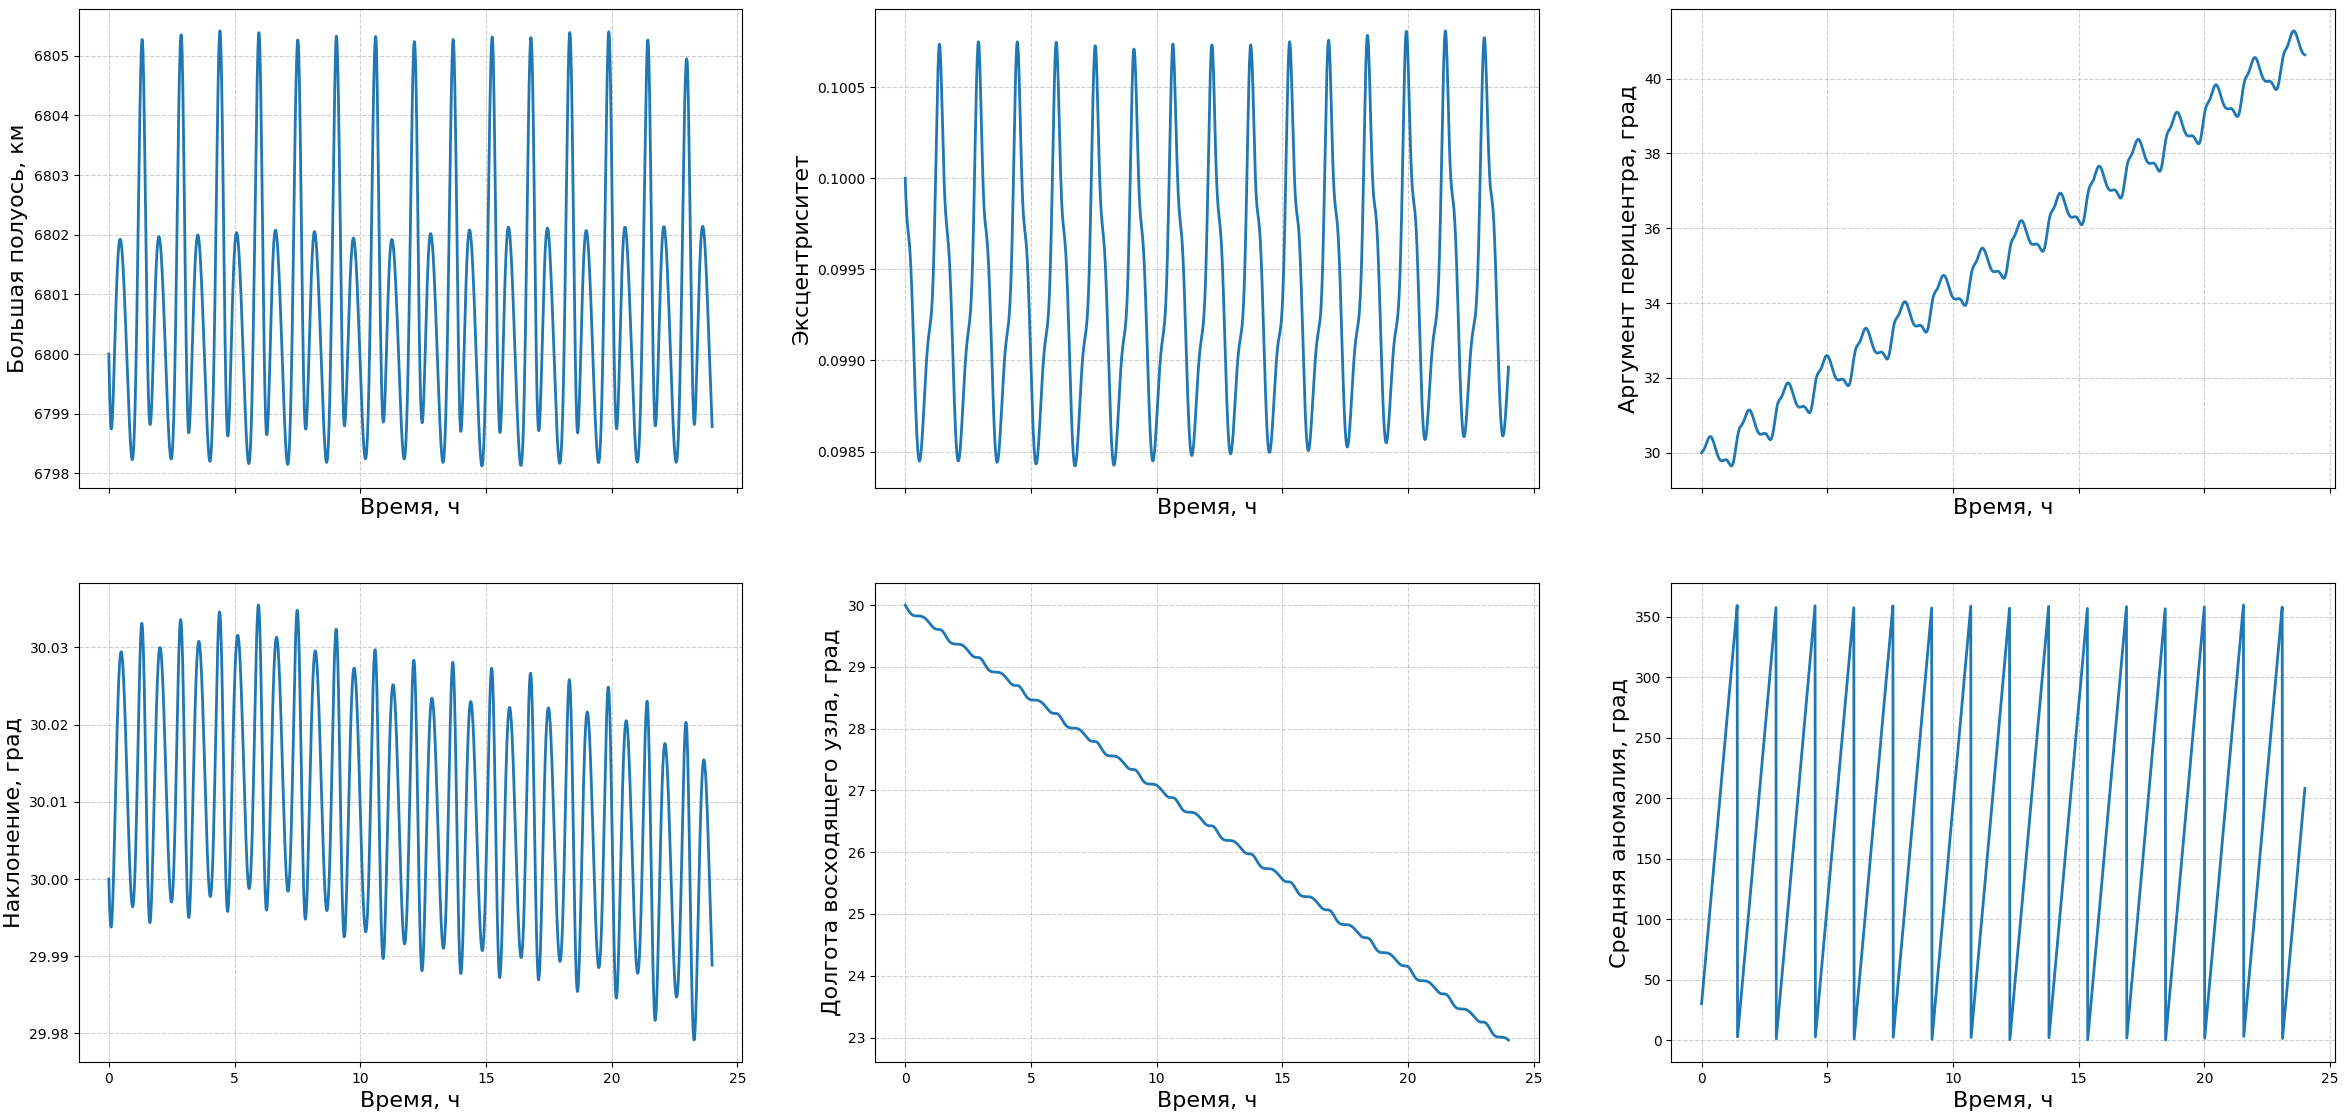
\includegraphics[width=1\textwidth]{images/1/real_motion.png}
    \label{fig:real_motion}
\end{figure}
\end{frame}

\begin{frame}{Движение КА в поле точечного потенциала}
\begin{figure}[h!]
    \centering
    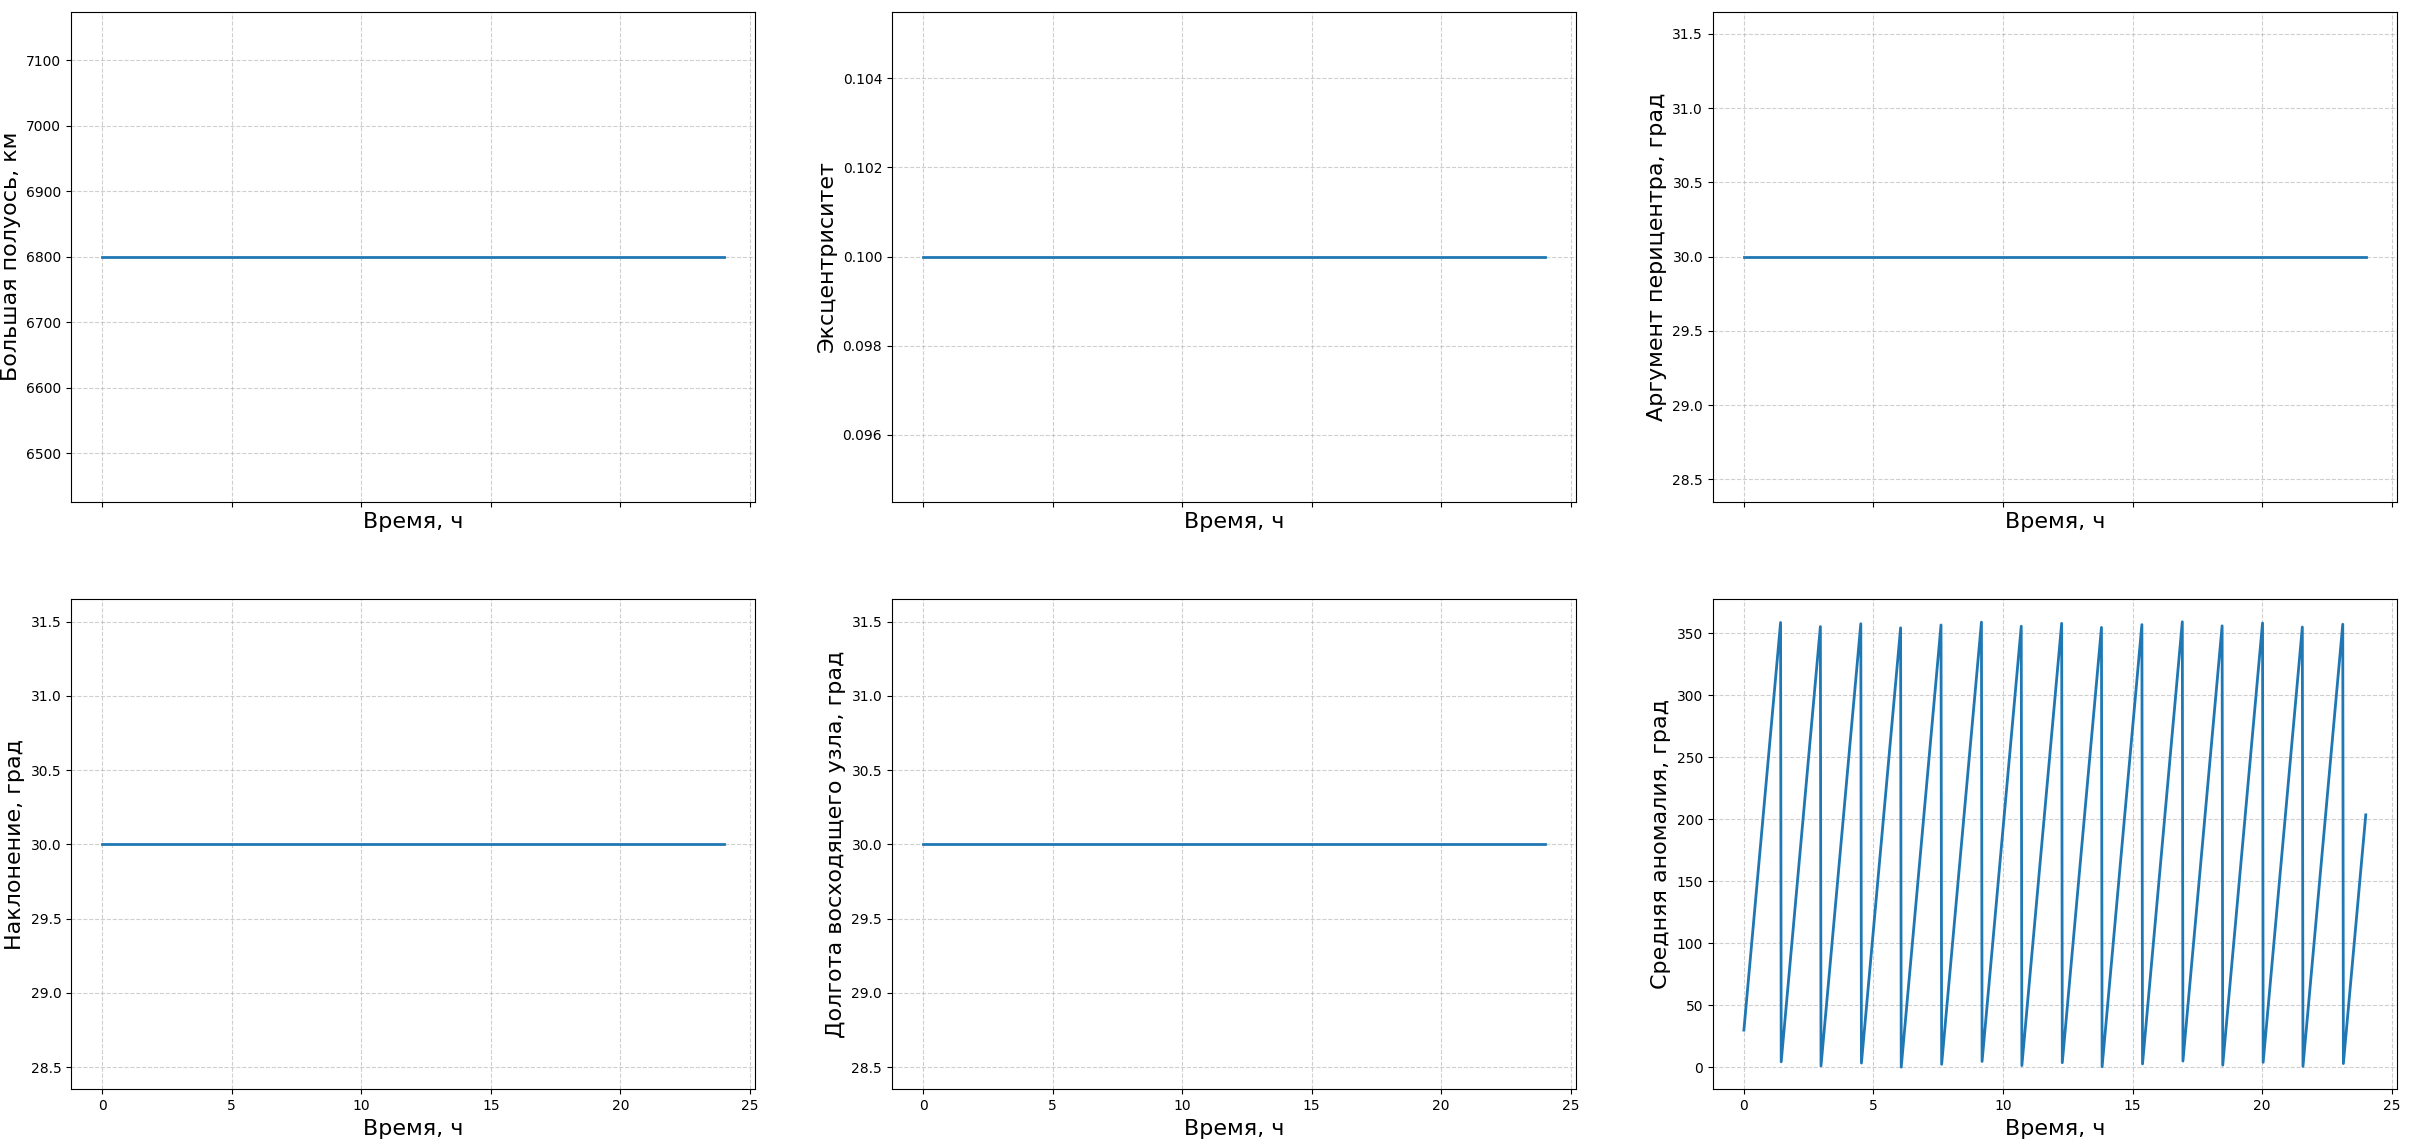
\includegraphics[width=1\textwidth]{images/1/main_force.png}
    \label{fig:main_force}
\end{figure}
\end{frame}

\begin{frame}{Постановка задачи перехода}
Рассмотрим обыкновенное дифференциальное уравнение и начальное условие
\begin{equation*}
    \dot{\mathbf{y}} = \mathbf{f}(t, \mathbf{y}) + \mathbf{u}(t),
\end{equation*}
\begin{equation*}
    \mathbf{y}(t_i) = \mathbf{y}_i = \left( \textbf{Э}_i, \nu_i \right)^T,
\end{equation*}
где $\mathbf{y}(t) = \left( \textbf{Э}(t), \nu(t) \right)^T$ --- вектор состояния, $\textbf{Э}(t)=\left( a(t), e(t), i(t), \omega(t), \Omega(t) \right)^T$ --- параметры кеплеровой орбиты, $\mathbf{f}(t, \mathbf{y})$ --- правая часть пассивного движения, $\mathbf{u}(t)$ --- управляющая функция. Необходимо найти такую управляющую функцию $\mathbf{u}^*(t)$, что функционал 
\begin{equation*}
    \int_{t_i}^{t_f} |\Delta V(\mathbf{u}^*(t))| dt \to \min,
\end{equation*}
будет достигать минимального значения при выполнении условия $\textbf{Э}(t_f)=\textbf{Э}_f(t_f)$, где $\Delta V = \Delta V(\mathbf{u}(t))$ --- функция характеристической скорости.
\end{frame}

\begin{frame}{Постановка задачи встречи}
Рассмотрим обыкновенное дифференциальное уравнение и краевые условия
\begin{equation*}
    \dot{\mathbf{y}} = \mathbf{f}(t, \mathbf{y}) + \mathbf{u}(t),
\end{equation*}
\begin{equation*}
    \mathbf{y}(t_i) = \mathbf{y}_i, \quad \quad \mathbf{y}_t(t_f) = \mathbf{y}_t,
\end{equation*}
где $\mathbf{y}(t) = \left( a(t), e(t), i(t), \omega(t), \Omega(t), \nu(t) \right)^T$ --- вектор состояния, $\mathbf{f}(t, \mathbf{y})$ --- правая часть пассивного движения, $\mathbf{u}(t)$ --- управляющая функция. Необходимо найти такую управляющую функцию $\mathbf{u}^*(t)$, что функционал 
\begin{equation*}
    \int_{t_i}^{t_f} |\Delta V(\mathbf{u}^*(t))| dt \to \min,
\end{equation*}
будет достигать минимального значения при выполнении условия $\mathbf{y} (t_f) = \mathbf{y}_t$, где $\Delta V = \Delta V(\mathbf{u}(t))$ --- функция характеристической скорости.
\end{frame}

\begin{frame}[allowframebreaks]{Источники}
  \begin{thebibliography}{9}
    \bibitem{Ovchinnikov}
    Овчинников М. Ю. Введение в динамику космического полета //М.: МФТИ. – 2016.

    \bibitem{Vallado}
    Vallado D. A. Fundamentals of astrodynamics and applications. – Springer Science \& Business Media, 2001. – Т. 12.

    \bibitem{Eliasberg}
    Эльясберг П. Е. Введение в теорию полета искусственных спутников Земли. – 1965.

    \bibitem{Baranov}
    Баранов А. А. Маневрирование космических аппаратов в окрестности круговой орбиты //М.: Спутник. – 2016.

    \bibitem{DiPrinzio}
    DiPrinzio M. Methods of Orbital Maneuvering. – American Institute of Aeronautics and Astronautics, Inc., 2019.
    
  \end{thebibliography}
\end{frame}

\end{document}
